\section{Description du système}

\begin{figure}
\begin{center}
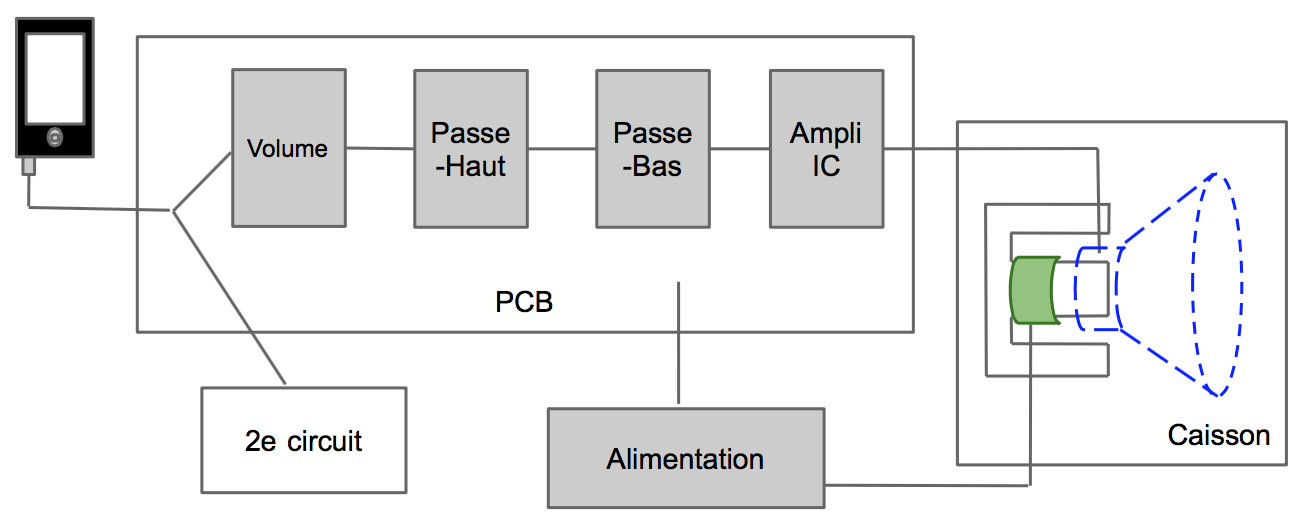
\includegraphics[width=\textwidth]{img/schemacomplet} 
\end{center}
\caption{Schéma général du système}		
\label{fig:schemacomplet}		
\end{figure}

Le système (voir figure~\ref{fig:schemacomplet}) est constitué de 2 parties principales : le circuit imprimé (PCB) et le caisson. 
Ces 2 parties ont été réalisées en double afin de pouvoir gérer un signal stéréo ou d'utiliser un des 2 baffles principalement pour les aigus et l'autre pour les basses. Le circuit de ces 2 hauts-parleurs est identique.
Le signal provenant du smartphone ou baladeur audio est transmis à la PCB grâce à une prise Jack.
La PCB est composée de 4 parties principales :
\begin{itemize}
\item Un récepteur, permettant le branchement du cable jack et permettant d'envoyer un des 2 signaux vers le seconde circuit imprimé.
\item Un potentiomètre, permettant le réglage du volume.
\item Un filtre passe-haut et un filtre passe-bas, permettants respectivement de limiter les basses et les aigus. Ces 2 filtres sont alimentés en +15\,\volt \, et -15\,\volt \, par une source de tension.
\item Un amplificateur, permettant d'amplifier 50 fois le signal de sortie.
\end{itemize}
Le signal à la sortie de la PCB est envoyée vers le caisson et en réalité vers la bobine mobile.
Le caisson peut se décomposer en 3 parties :
\begin{itemize}
\item L'électroaimant, permettant de créer un champ magnétique et donc de faire bouger la bobine mobile. Elle est alimentée par une source de tension de laboratoire.
\item La bobine mobile, permettant de faire vibrer la membrane.
\item La membrane, qui par son mouvement reproduit le son souhaité.
\end{itemize}
Les 2 caissons sont pour leur part différents, un des 2 à plutôt été conçu pour les aigus, il s'agit d'un petit haut-parleur de type ouvert. Le second à été conçu pour les basses, il s'agit d'un plus gros haut-parleur de type bass-reflex.